
\section{Evaluation of Project}
Evaluation of the project consisted of multiple stages ranging from verification of the functional requirements through simple black box testing to evaluation of refined mesh quality using methods provided by Dittmer \cite{DittmerMeshQualityMet}. 

\subsection{Validation Against Functional Requirements}
In order to validate the system against many of the functional requirements the system only needs to be run on several basic models with different input configurations. Having run the system on a range of different models results clearly demonstrates the systems ability to evaluate the quality of meshes using multiple refinement processes based on the stresses induced by the user and their categorisation of edges within the model. 

\subsection{Validation Against Non Functional Requirements}
Validation of non functional requirements was made simple due to the limited number of them, this was partly a consequence of the system not being designed for a specific user base resulting in expectations regarding the systems design to improve usability and guide interaction. It was also not possible to define the general accuracy and performance of the system during the requirement elicitation phase since this could only be determined once the required research and trial on the finished system gave indication to both of these. \\

\noindent
In the case of quality for the systems design and documentation evidence is present to indicate that this adheres to the requirements specified with the project submission containing detailed documentation in the form of a Deoxygen guide and sophisticated use of object oriented and functional software design as seen within the codebase. General applicability of functionality has also been demonstrated through evaluation using a variety of both models and conditions when performing simulations.

\subsection{Unit Testing}
Holistic evaluation provided evidence of the overall systems effectiveness however without verification of individual components it would not have been possible to assert the accuracy of the results produced. Unit testing was also conducted from within Visual Studio using the NUnit framework and structured as a separate VS project. This Guaranteed that the system was not able to interact with the tests and that testing was conducted through the class and function interfaces provided by the implemented solution. Tests were also grouped into classes with each test class corresponding approximately to one class within the system. Each test class then contains a number of test functions each of which performing the asserts necessary to deem its associated function as correct. This layout provided clear traceability from each item of function to its associated test making assessment of the test coverage much easier. Appendix B shows the visual studio test explorer containing the various tests. \\


\subsection{Software Quality and Management}
The quality of the design and implementation of the system reflects my experience not only as a computer science undergraduate but as a developer with one year industrial experience, although not directly effecting the execution of the program properties such as appropriate variable naming, loose coupling of classes, use of abstractions and descriptive error messages make the software easier to read and debug for any potential future developers. \\

\noindent
Visual Studio also enabled calculation of various software quality metrics for the code base automatically. This made selecting parts of the codebase for refactoring much easier when time was allocated for this. Upon completion of the project the average maintainability index across all modules was 75 with the lowest score for any high level module being 60 and the highest 92. According to the Microsoft Developer Network (MSDN) website code with an index of between 0 and 9 indicates low maintainability, 10 to 19 indicates moderately maintainable and 20 to 100 high maintainabilty \cite{VisualStudioMaintainIndex}. \\

\noindent
In order to ensure progress was responsibly backed up and new features easily managed a private Github repository was set up and all progress made to the project pushed every couple of days. This proved invaluable on at least one occasion where a bug was accidentally introduced and despite efforts could not be removed manually. 


\subsection{Documentation}
The process of continuously writing descriptive documentation was important to the success of the project and was treated as an integral part to meeting the goals of the project development methodology which aimed to reduce the systems complexity and improve readability. Through the writing Doc comments corresponding to every function within the codebase it was possible to generate documentation files automatically through use of the tool Doxygen. This allows anyone with the solution to view descriptions of each of its functions either in the codebase or alternatively through the manual produced automatically by Doxygen. \\ 

 

\subsection{Evaluation Of System For Model Simulations}
%To demonstrate the systems applicability to a variety of real engineering problems demanded the creation of several models resembling basic equivalents of real structures that are often analysed by FE methods.

As a system designed to facilitate analysis of hybrid meshing techniques the ability conduct detailed evaluation for a set of hybrids over multiple simulations demonstrates successful generality. \\

\noindent
Three models have been created in total as simulation input by which to test the overall refinement system. With each of the three models being a general simplification of some more complex model that could be expected within an industrial engineering setting. Before any refinement occurs each model has a manually constructed low fidelity mesh built using LISA's graphical user interface. Each model also has a set of forces applied to it which are required to induce stress within the simulation along with various constraint surfaces as described under the Motivation and Background section. \\ 

\noindent
Another important aspect of designing the evaluation process was deliberate  variation of inputs for each of the refinement processes. This was particularly important in the case of the heuristic method where results could dramatically vary depending on the quality of the edge description input. The effects of edge variation is observable both in execution times for the simulations and in the systems ability to mesh accurately where required as seen in Figure 14 and the mesh structure in appendix F. \\ 

\noindent
Four sets of of edges were consequently constructed for each of the models and given classifications of ``Best'', ``Good'', ``Ok'' and ``Poor'' With the following as general guidelines for defining each set: \\

\noindent
\textbf{Best: } Approximately five edges specified directly over or adjacent to those areas of known high stress within the model - input potentially generated by a user with a high degree of expertise in evaluating the specific type of structure. \\ 

\noindent
\textbf{Good: } Approximately three edges over or close to areas of high stress within the model - input potentially generated by a user with a high degree of general FE experience although potentially not specific to that type of structure. \\ 

\noindent
\textbf{Ok: } Three to five edges some near high stress and other not - representing a user with some experience but by no means an expert. \\ 

\noindent
\textbf{Poor: } Three to five edges none of which are close to areas of high stress - representing input as would be generated by an inexperienced user new to FE stress analysis. \\ 

\noindent
As someone who would identify as an inexperienced user determining the areas of high stress in advance was important in order to successfully develop rule sets which satisfied each of these categories  for each of the different simulations. The system was therefore initially run for each model without a heuristic component in order to provide some indication of what edges might be described for each set. Having obtained the four edge sets for each of the three models both the heuristic and hybrid simulations using each set and thus providing data on the performance of these methods based on different levels of user expertise. \\

\noindent
A clear drawback of not having the edge sets defined by an experienced FE engineer is a lack of a guarantee that the edge sets chosen by me accurately represent those similar to what would be specified by a typical user of the system. At best it can be asserted that the sets represent a range of deviations from the theoretical ideal for the edge specifications which it is reasonable to expect from users with varying degrees of skill. Consequently it is only possible to objectively judge each of the different sets on the basis of the results they produce. These results for the different specifications cannot be claimed to represent the output mesh of a user group.\\ 

\noindent
The results below for the suspension bridge model reveal several trends present across the different refienement methods. The suspension bridge model consists of 196 quad4 elements and 212 nodes which can be considered coarse given the size of the structure. Four constraint points were specified at the base of each supporting column and strong forces of applied across the structure along the negative x axis. \\ 


% show angle and runtime

\begin{figure}[H]
\centering
\begin{subfigure}{.5\textwidth}
  \centering
  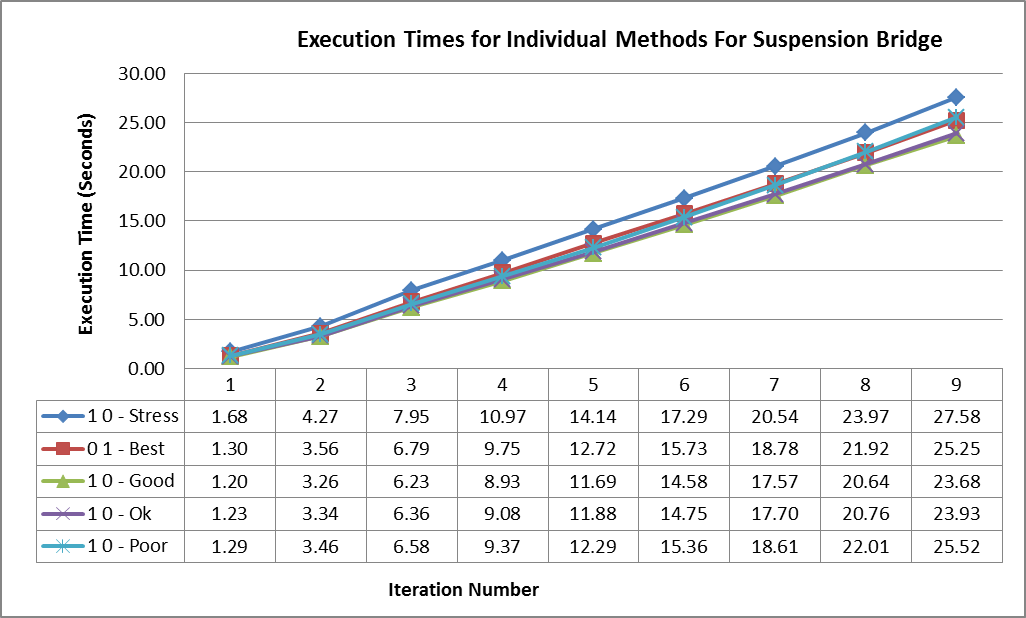
\includegraphics[width=0.9\linewidth]{../Graphics/Graphs/SingleMethods/ExecutionTimes.png}
  \caption{Time taken to complete each iteration using the different methods}
  \label{fig:sub1}
\end{subfigure}%
\begin{subfigure}{.5\textwidth}
  \centering
  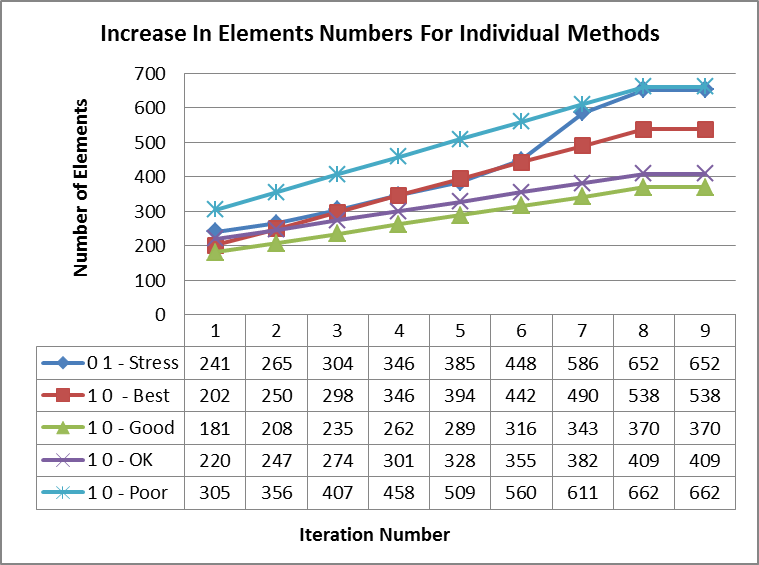
\includegraphics[width=0.75\linewidth]{../Graphics/Graphs/SingleMethods/NumberOfElements.png}
  \caption{Increase in number of elements for each of the individual refinement methods}
  \label{fig:sub2}
\end{subfigure}
\label{fig:test}
  \caption{Execution time increase compared to the amount of information revealed for the different approaches}
 \end{figure}
 
\noindent
Looking at the the maximum conner angles within the elements in figure 15 below it can be see that the general element quality improves over time with the greatest rate of improvement occurring during the first few iterations of each method before decreasing as the average for the mesh increasingly approaches the optimum, which for elements of type  quad4 is 90 degrees. This data indicates that all of the methods tend to reduce skew present in initial meshes when performing refinement. This is useful to know since it suggests the solver is able to correctly calculate the correct stress results across the model based on the mesh formulation. \\ 

\begin{figure}[H]
  \centerline{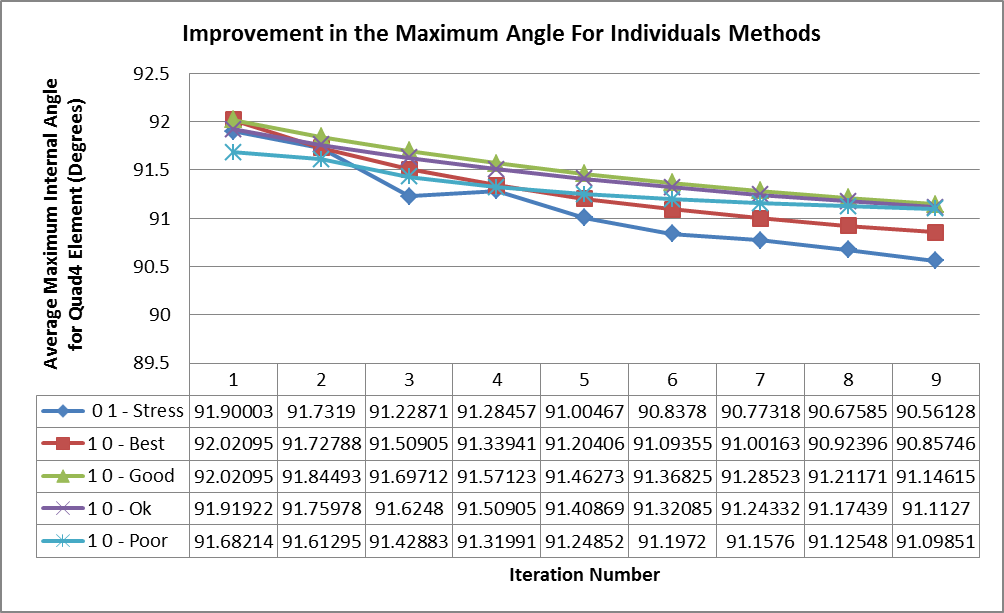
\includegraphics[width=110mm, scale=1]{../Graphics/Graphs/SingleMethods/AngleImprovements.png}}
  \caption{Approaching the ideal quad4 geometry for simulation data accuracy of 90 degrees using refinement with each of the different methods}
  \label{fig:sub1}
\end{figure}  

\noindent
A key realisation having calculated the average maximum angles for the different methods was although Dittmers metrics helped to indicates that the results produced by the solver are accurate they do not actually demonstrate one methods ability to mesh in more desirable areas than another. It was therefore clear that an alternative metric need to be devised to show this. A simple solution which proved effective was simply to calculate the average stress value across all nodes created during refinement under a particular method. graphing this over iterations gave an accurate representation of each methods effectiveness with the average being reduced if a method poorly selects an area under which to refine and increased if meshing occurs exclusively in areas of concentrated stress. \\

\noindent
Evaluating each of the individual methods using this metric produced the following results: \\ 


\begin{figure}[H]
  \centerline{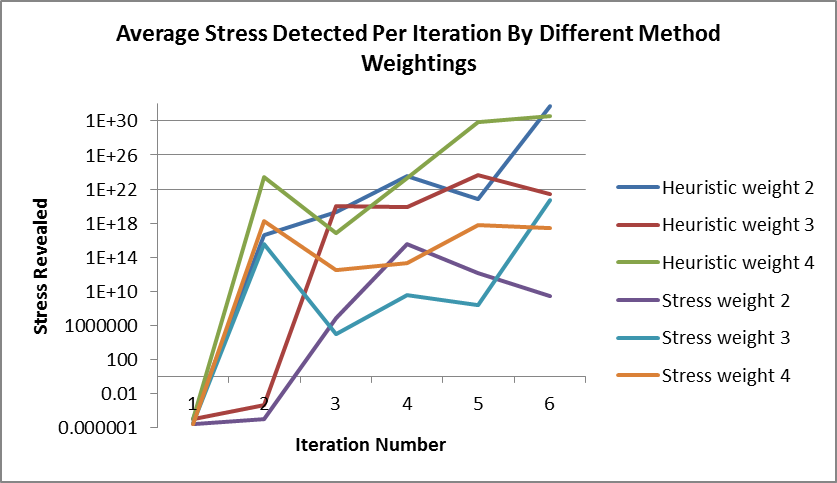
\includegraphics[width=110mm, scale=1]{../Graphics/Graphs/AverageStressDiffHybrWeightings.png}}
  \caption{Increase in element count for the various refinement methods over forty iterations}
  \label{fig:sub1}
\end{figure}


% graphs for improvement of different methods.
\noindent
Having completed analysis for each of the individual methods it was possible to run some hybrid strategies for each of the models, with successful execution of these models producing results that indicate rapid overall improvement with regards to finding stress. 

% seen as quickly improving within the first few iterations, most likely as a result of the refinement producing ele

\noindent
The highly exponential rate of improvement in these results was surprising to the extent that for a period it seemed as though the results must be incorrect. Re execution of the model with varying configurations including reduced force and constraints revealed no difference to this aspect of the results however. Conducting additional research then revealed that this is not in fact an uncommon as a property of stress gradients within FE models as stress will trend towards infinity at points of serious weakness within a design given the opportunity. Considering the approaches used the stress refinement method will inevitably continue to focus on these areas whilst the heuristic approach is unlikely to \cite{StressConcerntration}.  \\

\noindent
For designs where there is then a clear weakness the increasing speed at which meshing can be focused using stress refinement approach will clearly outperform that of a more general heuristic method. The extent to which this is true for a model varies however and so looking for more general weaknesses may still favour a different approach that will provide significant speed up during the initial few iterations when there is no clear stress point that can be identified. Figure 16 below shows the bridge model undergoing relatively high stress at various points across the model but with exponential increase at specific points where structures join one another. \\ 


%../Graphics/BridgeCrossLoadingStress/bridgeStressBasic.png
\begin{figure}[H]
\centering
\begin{subfigure}{.5\textwidth}
  \centering
  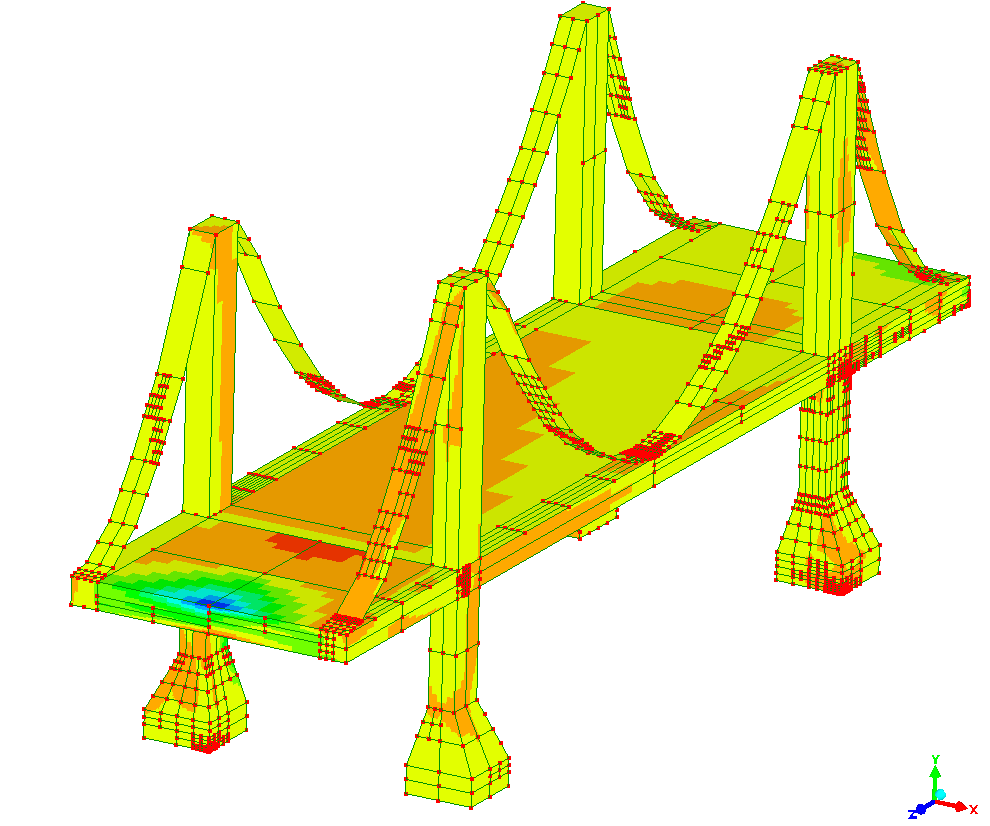
\includegraphics[width=0.9\linewidth]{../Graphics/BridgeCrossLoadingStress/Hybrid-best-3-2.png}
  \caption{Stress Revealed through the initial highly coarse bridge mesh without running any iterations for either method}
  \label{fig:sub1}
\end{subfigure}%
\begin{subfigure}{.5\textwidth}
  \centering
  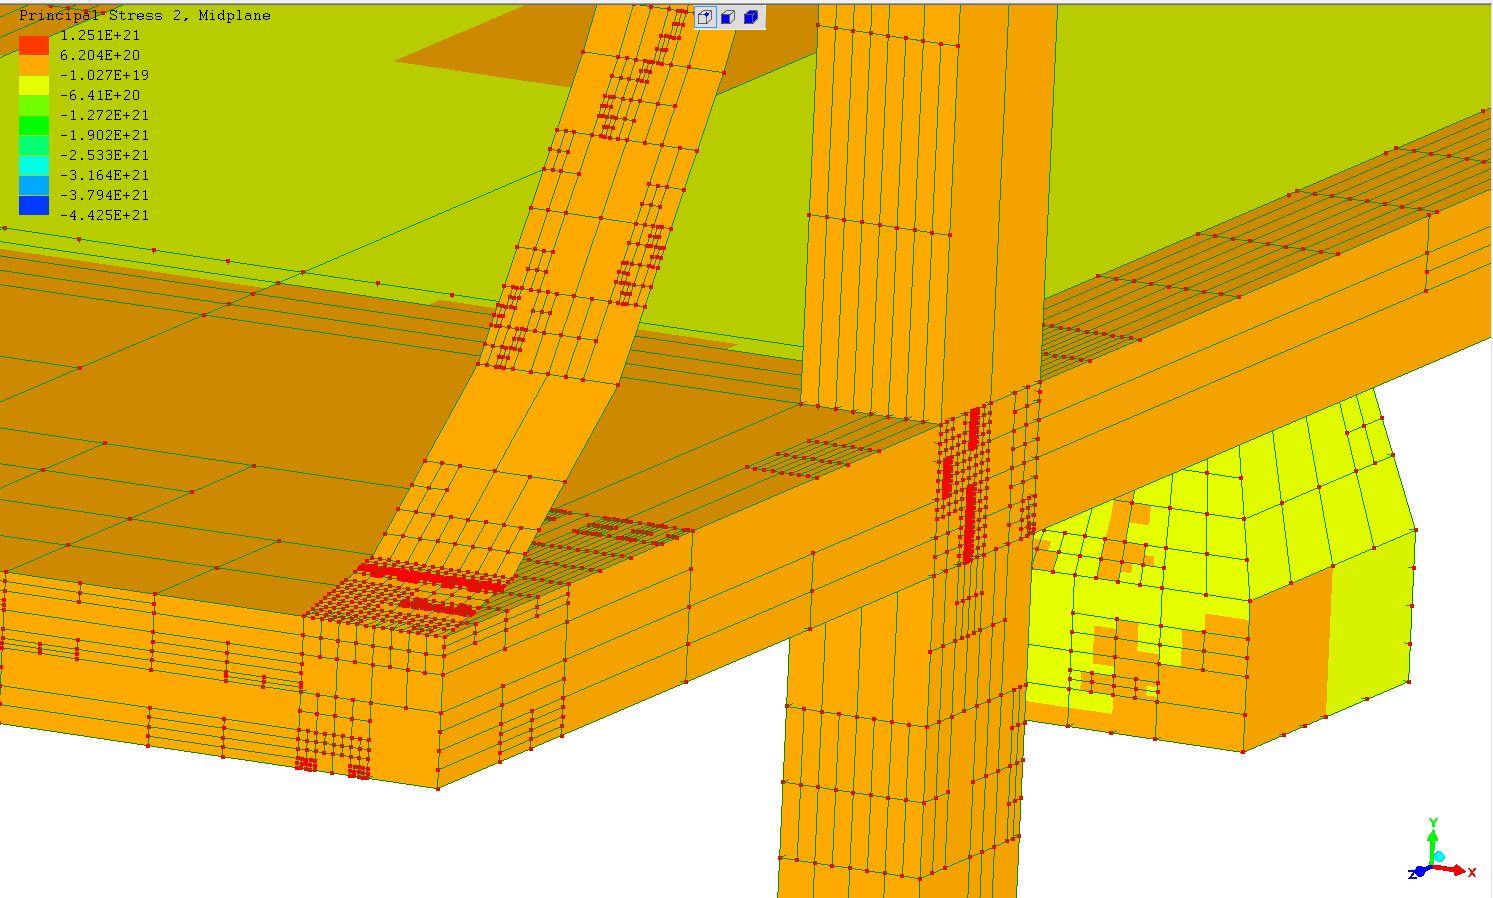
\includegraphics[width=0.9\linewidth]{../Graphics/BridgeCrossLoadingStress/BridgeCrossLoadingStress6-3-2.png}
  \caption{Stress revealed within model after just 4 iterations with a heuristic stress method weighting of 3-2, edge heuristics also considered good in this case}
  \label{fig:sub2}
\end{subfigure}
\label{fig:test}
  \caption{Execution time increase compared to the amount of information revealed for the different approaches}
 \end{figure}



%Results obtained from this model can be used for verification against a comparable system the meshes for both the paper mill and cylinder structures have been designed to closely resemble the input data originally used by Dolsak as input for training the ILP when generating the rule set, \cite{DolsakPaper91} although there is little numerical data on the results of simulation with these meshes. 
%Comparing the results for these models against those obtained by Dolsak provides a means of evaluating both the implementation of the ILP generated rules within system in addition to providing general models for which  the results obrained for the suspension bridge can be compared.
%suspension bridge goes beyond Dolsak models. 
%\cite{}
%\noindent
%The two additional models one being a section of a paper mill disk and another being half of cylinder were both based on designs specified within Dolsaks paper 
% \cite{SuspensionBridgeMeasurements}.

%independently of one other. This provided data on the performance of each approach making it easier to evaluate the results of hybrid executions later.
%evaluate both approaches before attempting to combine the two. Testing each method

%\noindent
%For stress refinement the varied parameter was the threshold used to determine whether elements were considered under high stress and should be further refined. The main consequence of varying this parameter was change in both the node count and the programs runtime as can be seen in Figure 14a. Despite time complexity for subdivision being $O(n^2)$ for all methods using a low threshold results in large values of n and consequently a rapid increase in both runtime and element count. \\




\noindent
Looking at the metric and the resulting meshes it is clear that the system quickly identifies areas under very high stress with both approaches after just a few iterations, with meshing being highly focused on those areas and consequently a rapid increase in the average stress covered by the elements in the model after only two iterations. \\ 

%say something about how actually you want a bit of distribution

\noindent
Comparing the amount of improvement performed by both the stress and heuristic refinement processes with varying weightings that in general heuristics performed better than stress refinement although interestingly more weighting did not necessarily correlate to better results as can be be seen with heuristic weighting of two doing a better job than weighting four in the final iteration. \\




\noindent
Effective comparison of the two methods indicates that the system works as a tool by which comparisons of different refinement methods can effectively be made. 

%


%\subsubsection{Evaluation Issues}
%A significant issue faced in attempting to demonstrate the effectiveness of the system was to provide an indication of how well the system worked without taking into account the ability of the user who may be providing the edge rules for a particular model. Not taking this into account would result in an inaccurate representation of its ability.

\subsection{Strengths and Weaknesses}
The resulting system successfully satisfied both the functional and non functional requirements in addition to providing insights into the possibilities of a hybrid technique for effective finite element meshing, something that was optimistic at the start of the project but highly desirable. The project was well managed with all of the objectives being delivered as per the initial time plan. Quality was also maintained throughout the project by the application of good software engineering practice. \\

\noindent
One of the greater strengths of the finished system was its modular architecture which allows for a great amount of potential extendibility in the future. Although little focus has so far been given to the systems usability it could be developed and distributed as a public tool for experimentation with hybrid meshing with limited additional effort. \\

\noindent
Another strength of the system is its ability to accept any heuristic definition in terms of edges within a mesh structure. Theoretically this means the final system is also capable of using the same types of edge specifications for any type of FE analysis such as fluid flow or heat transfer given a corresponding rule set by which to mesh with. \\


\noindent
A downside of the current design is the need for the user to manually specify the edges by the user directly into the JSON input file which is both time consuming and prone to error despite the relatively small size of the models analysed in this dissertation. Comparing the size of these with those used in industry it is clear that this process is simply not practical for engineers conducting FE analysis. To change this better tools are required that will allow engineers to automatically generate edge specifications quickly, most likely through some GUI or a bespoke high level language capable of combining knowledge about the mesh structure and different types of edges to generate specific rules. Again this is beyond the scope of the project and would likely be a dissertation in its own right. \\


\noindent
Although the system had a strong subsystem and class level architecture many of its weaknesses could be attributed to needing to prioritise the ability to perform rapid prototyping over efficient implementation of the various algorithms and methods described in this dissertation. Much of this a consequence of overusing the functional programming capabilities within the C\# LINQ library. Widespread adoption of functional programming practices was stated as a desirable aspect of the final system implementation within the non-functional requirements. This has largely been adhered to with  higher order and lambda functions widespread throughout the codebase. In the later stages of the project it became apparent however that in many cases reliance on these features resulted in reduced readability and performance for many of underlying algorithms described in this dissertation. \\


% Overall the project met all its initial requirements laid out in both the objectives and its requirements.
% Sould have done test driven development to ease testing at the end


\subsection{Evaluation summary}
Having used the system to successfully evaluate a range models we can see that multiple methods can successfully be combined simultaneously with analysis possible for each of the individual methods and the resulting hybrid.